
\documentclass[12pt, reqno]{amsart}
\usepackage{amsmath, amsthm, amscd, amsfonts, amssymb, graphicx, color}
\usepackage[bookmarksnumbered, colorlinks, plainpages]{hyperref}
\usepackage{graphicx}
\textheight 22.5truecm \textwidth 14.5truecm
\setlength{\oddsidemargin}{0.35in}\setlength{\evensidemargin}{0.35in}
\setlength{\topmargin}{-.5cm}
\usepackage[ backend=biber,style=alphabetic, sorting=ynt]{biblatex}
\addbibresource{references.bib}
\begin{document}
\setcounter{page}{1}

\centerline{}
\centerline{}


%------------------------------------------------------------------------------

\title[EMP Modelling]{Modeling Electromagnetic Pulse Interactions with Earth's Ionosphere and Magnetic Field}
\author[]{Atlas Hussey}

%------------------------------------------------------------------------------------

\begin{abstract}
An electromagnetic pulse can be propagated through a couple of sources, namely lightning and nuclear blasts. Satellites such as the FORTE and GPS satellites can detect these pulses as they pass through Earth's ionosphere. However, the ionosphere distorts the signal produced by the electromagnetic pulse. Using Fourier transforms, I am able to model the distortion of the electromagnetic pulse caused by the ionosphere in order to gain a better understanding of it.  

\end{abstract} \maketitle

%------------------------------------------------------------------------------

\section{Introduction}

\noindent In order to propagate radio waves, one must first generate a strong electric current.
In an AM radio tower, the wave is constantly powered by a 50,000 watt electric source
running throughout the tower, moving the electrons. Although radio towers are constant,
other sources of radio waves can be impulsive, such as nuclear blasts.

\noindent When a nuclear weapon goes off, it releases a large amount of gamma radiation, which strips atoms of their electrons. This causes the free electrons to suddenly be expelled, propagating a strong burst of radio frequencies known as an electromagnetic pulse, or EMP. An electromagnetic pulse such as this can be highly destructive, as a sudden surge of electromagnetic energy can overload electronics and power grids. 

\noindent Lightning strikes can also produce a similar pulse due to the rapid discharge of electrons during a strike producing $10^6$ volts per meter. Lightning is also much more frequent, striking the earth around 1000 times per second. However, lightning is only capable of producing a signal similar to a nuclear blast under certain conditions. Satellites such as the FORTE satellite and GPS satellites are built with an EMP detector to analyze these signals, initially to monitor compliance with nuclear test ban treaties, but now to study lightning from space. In this project, I intend to take a simplified approach in modeling how Earth's ionosphere and magnetic field affect the frequency signature of an electromagnetic pulse. 

%------------------------------------------------------------------------------------

\section{Background}

\subsection{Earth's Ionosphere}

\noindent As an EMP passes through the ionosphere, it encounters a varying amount of free electrons. These electrons absorb some of the energy of frequencies in the signal, distorting it. This distortion causes higher frequencies to be received tens of microseconds later than the original pulse, and the lower frequencies show up hundreds of microseconds later. The lowest frequencies are unable to penetrate Earth's ionosphere entirely and instead are reflected back down to Earth's surface.

\noindent The extent of this delay is dependent on the total electron density of the atmosphere. The total electron density depends on the amount of ionizing solar radiation the ionosphere receives; more radiation in cases such as solar flares or Earth's surface facing the Sun increases the electron density.

\subsection{Earth's Magnetic Field}

\noindent Earth's magnetic field also changes how the signal can be read through the ionosphere. At first glance, the initial signal appears to be linear. While that may be true, the signal is also the sum of two polarizations, one that rotates counterclockwise (right-circular), another that rotates clockwise (left-circular). Earth's magnetic field separates the signal into these two "modes" that travel through the atmosphere at different speeds.

%------------------------------------------------------------------------------------

\section{Methods}

\subsection{Modeling the Initial Signal}
\noindent Whereas a radio signal appears as a sinusoid comprised of one frequency,
an EMP source contains many frequencies,  and usually has a fast rise and a slower fall in frequency. The rise and fall are both exponential functions, therefore the shape is known as a "double exponential". There are several ways to model double exponentials, but I used this equation:

\begin{center}
    $d(t)=A\frac{e^{t-t_0*t_r}}{1 + e^{t-t_0*t_r + t_f}}$
\end{center}

\noindent Rise and fall times are given in units of microseconds, so my signal had a rise $(t_r)$ of 0.01 microseconds and a fall $(t_f)$ of 0.4 microseconds. I modeled the pulse at 20 microseconds. The data points are in increments of nanoseconds, so I used a time frame of $2^{20}$ nanoseconds
which is roughly equivalent to 1050 microseconds.

\begin{figure}[h]
    \centering
    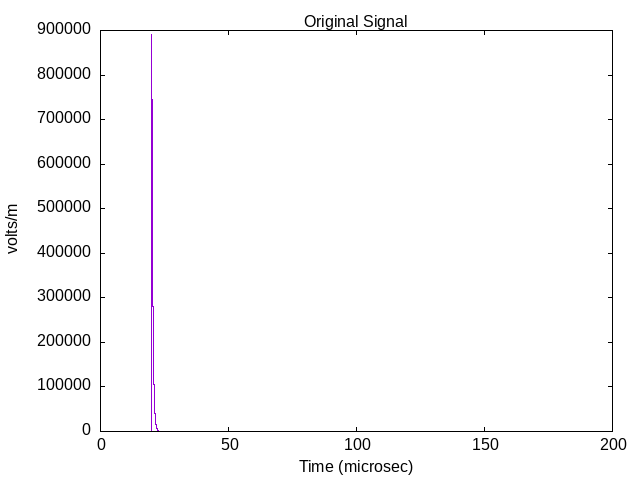
\includegraphics[width= 0.6\textwidth]{emp_original_signal.png}
    \caption{\small The initial EMP signal without interference from Earth's Ionosphere.}
    \label{fig:test-08}
\end{figure}

The faster the signal rises, the more powerful the frequencies in the electromagnetic pulse are.

\subsection{Fourier Transforms}
In order to properly simulate and analyze the changes Earth's ionosphere and magnetic field make to the signal, we must break the signal down into its frequencies. This can be done using a Fourier transform. A Fourier transform takes however many points there are in the signal, usually for the signal at every nanosecond, and multiplies each point by a sinusoid, as a singular frequency appears as one. It then plots the amplitude of each sinusoid into another graph to show how much power each frequency has. The Fourier transform utilizes Euler's formula $e^{i_x} = cos(x) + i*sin(x)$
to break down the complex sinusoidal signals into their real (cosine) and imaginary (sine) parts.Fourier transforms are quite useful in revealing frequencies as shown in the following figures:

    \begin{figure}[h]
        \centering
        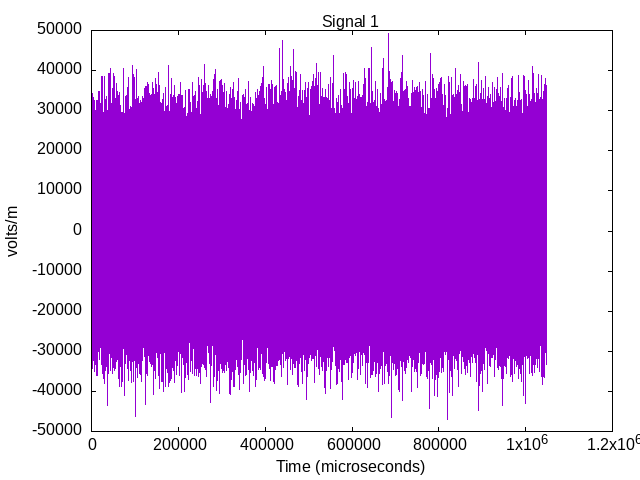
\includegraphics[width=0.6\textwidth]{test_08.png}
        \caption{Test data}
        \label{fig:test-08}
    \end{figure}
        \begin{figure}[h]
        \centering
        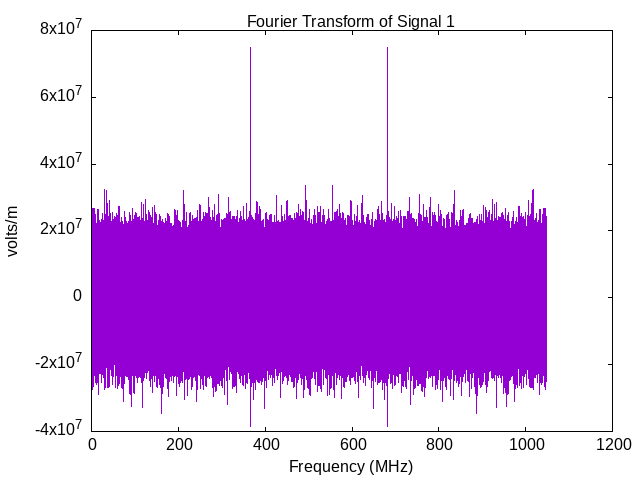
\includegraphics[width=0.6\textwidth]{fft_test_08.png}
        \caption{Fourier transform of the test data that reveals hidden frequencies}
        \label{fig:fft-test-08}
    \end{figure}

In the time domain, the frequency is quite low, so it gets buried under numerical noise. However, because the Fourier Transform multiplies the magnitude of the frequency for every time it occurs ($2^{20}$ nanoseconds), the frequency ends up having a lot of power.

\subsection{Symmetry}
\noindent In the array output by the Fourier Transform, the DC term is written first, and is located where the frequency is equal to zero. The DC term is the average of all frequencies in the Fourier Transform. This is then followed by all of the positive frequencies, then the Nyquist frequency, which is the highest positive frequency in the dataset. Finally, in reverse numerical order, the negative frequencies follow. For example, if you were to take 1024 data points along a signal, the Nyquist would appear at point 512. The function also exhibits Hermitian Symmetry, that is, the negative frequencies are the complex conjugates of the positive frequencies. 

\subsection{Aliasing}
\noindent Something to be mindful of when performing Fourier Transforms is a process called aliasing. In a signal, all frequencies must be included. However, we can only view a certain window of frequencies, so signals outside of the window of frequencies tend to "wrap around". For example, if we were to take a Fourier Transform of a signal with a high amplitude frequency at 700  MHz, yet we were only able to view frequencies up to 512 MHz, the frequency would show up at both 700(-188 MHz) and 188 MHz due to Hermitian symmetry. 
\\ 
Aliasing also occurs in the time domain. This is problematic, especially when the signal goes through the ionosphere and the lowest frequencies take hours to arrive.

    \begin{figure}[h]
    \centering
    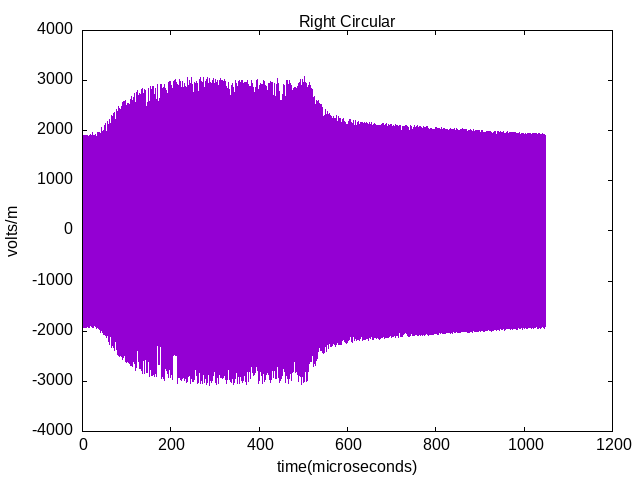
\includegraphics[width=0.8\textwidth]{time-aliasing.png}
    \caption{Aliasing in the time domain. The aliased frequencies add amplitude to the existing frequencies. A common indicator of aliasing is when the Nyquist or last frequency of a signal is not at or near zero. }
    \label{fig:time-aliasing}
    \end{figure}
    
\\
\\
\noindent To prevent aliasing when calculating the shift in frequencies caused by the ionosphere, I used a simple highpass filter. In the interest of time, the highpass filter I used set the amplitude of the lowest 7500 frequencies to zero. Such a simplified highpass filter is not completely accurate as to how the satellite reads the frequencies; the satellite tends to have a more gradual decrease in frequencies it can measure.

\subsection{Phase}
\noindent Earth's ionosphere affects the phase of the frequencies of an EMP. The phase dictates where and when the frequency will appear in a plot. The phase delay caused by Earth's ionosphere can be expressed as $e^{-i \Delta \theta}$ where $\Delta\theta$ is the change in phase. To calculate the phase delay caused by Earth's ionosphere I used this formula which is a simplified version of the formula used to calculate ionospheric delay.

\begin{center}
    \large$\Delta \theta = \frac{-8445 *STEC}{2\pi f}$
\end{center}

\noindent The STEC is the slant "total electron content", that is, the electron column density along the path the signal takes, given in units of $10^{16}$ electrons/$m^2$. It is typically between the ranges of 5 and 100.
\\
\\
\noindent Once the phase delay is applied, I then take the inverse Fourier transform of the signal, which, as the name suggests, expresses a function of frequency in the time domain.
As a signal in the time domain, it should have almost no imaginary power. To calculate the changes Earth's magnetic field make to the signal, I expressed $\Delta \theta$ as this function where it also calculated the cosine of the angle at which the signal entered Earth's ionosphere.

\begin{center}
   \Large $\Delta\theta= \frac{-8445*STEC}{2\pi f (1 \pm \frac{17.5Bcos(\delta)}{f})}$
\end{center}

\noindent I set the cosine to 0.125 radians. I evaluated the signal twice, one to calculate the right-circular mode (with the - sign) and the other to calculate the left circular (with the + sign).
Interestingly enough, the equations for the right and left circular are the opposite of one another in the southern hemisphere.

%------------------------------------------------------------------------------------

\section{Results and Discussion}

\begin{figure}[h]
    \centering
    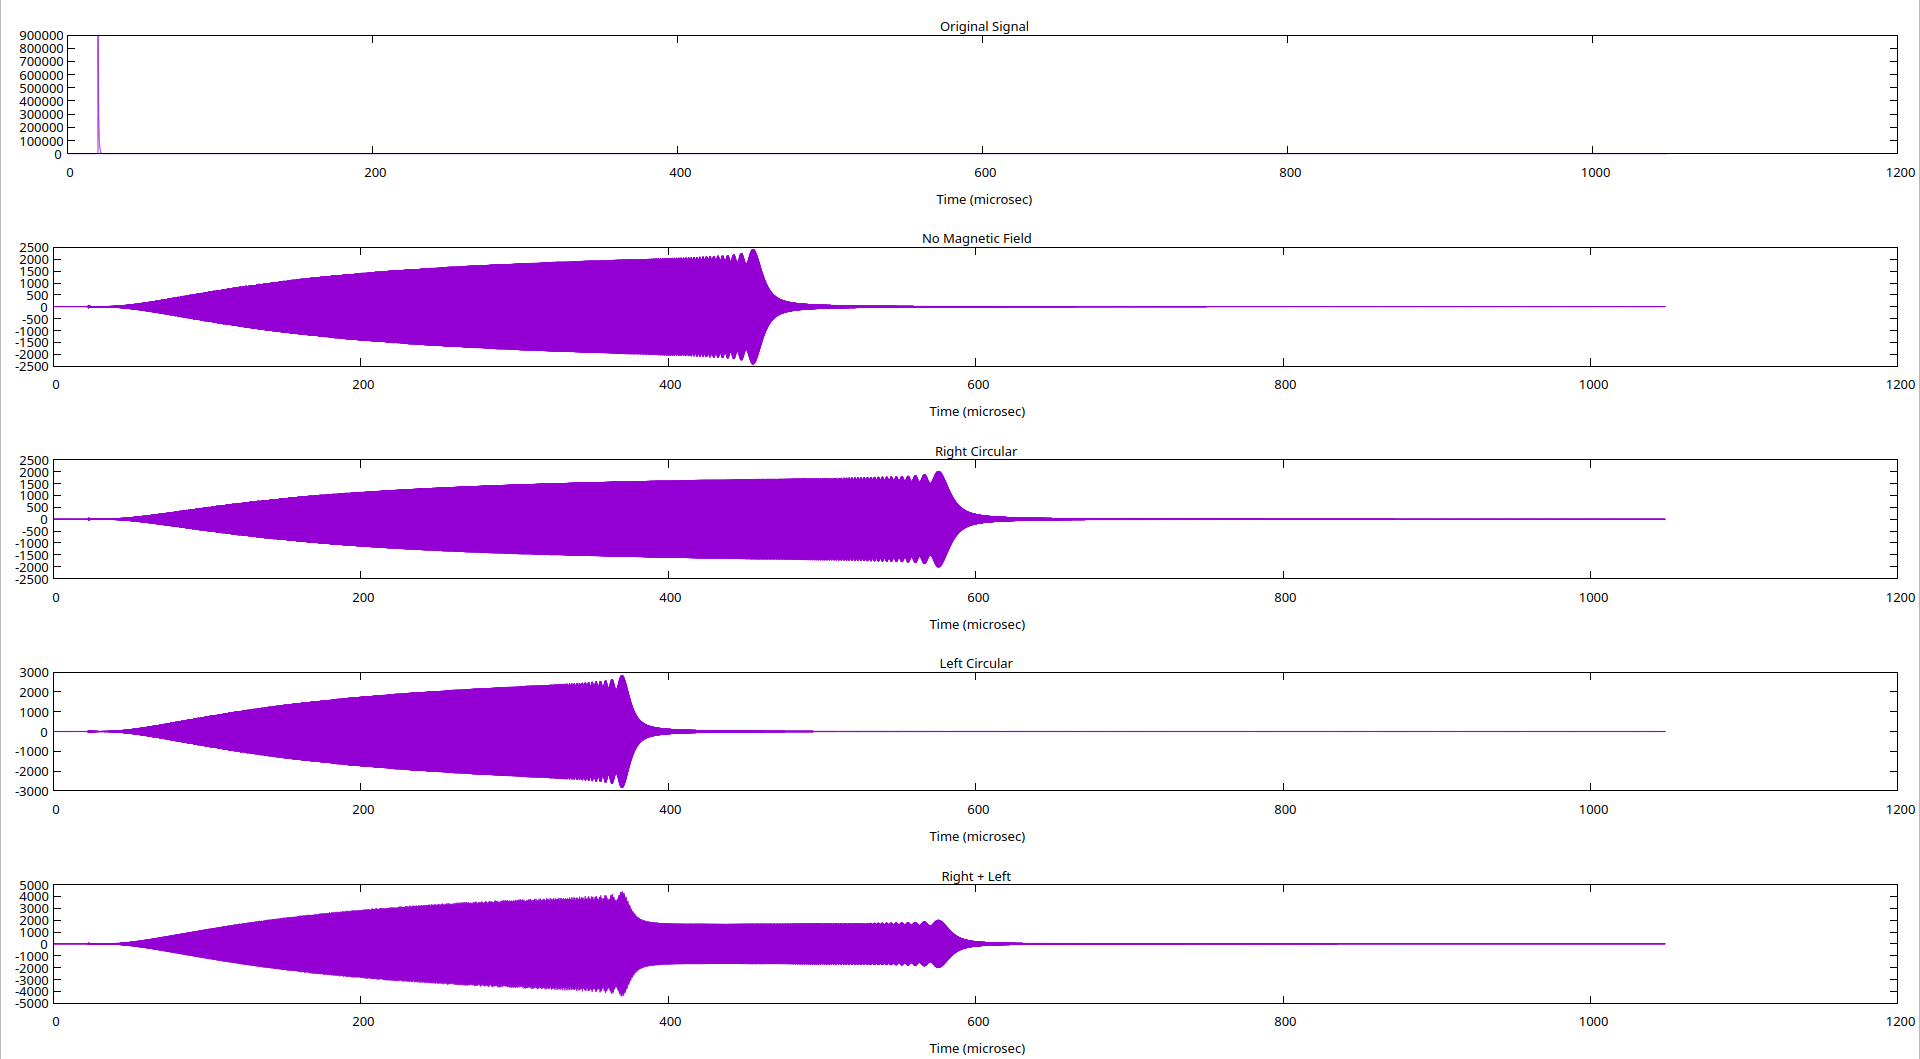
\includegraphics[width= 0.9\textwidth]{signal_final_results.png}
    \caption{\small Comparison of the original signal and the signal through the modeled ionosphere: right-circular, left-circular, a sum of the two, and without the magnetic field}
    \label{fig:signal-final-results}
\end{figure}

 \begin{figure}[h]
    \centering
    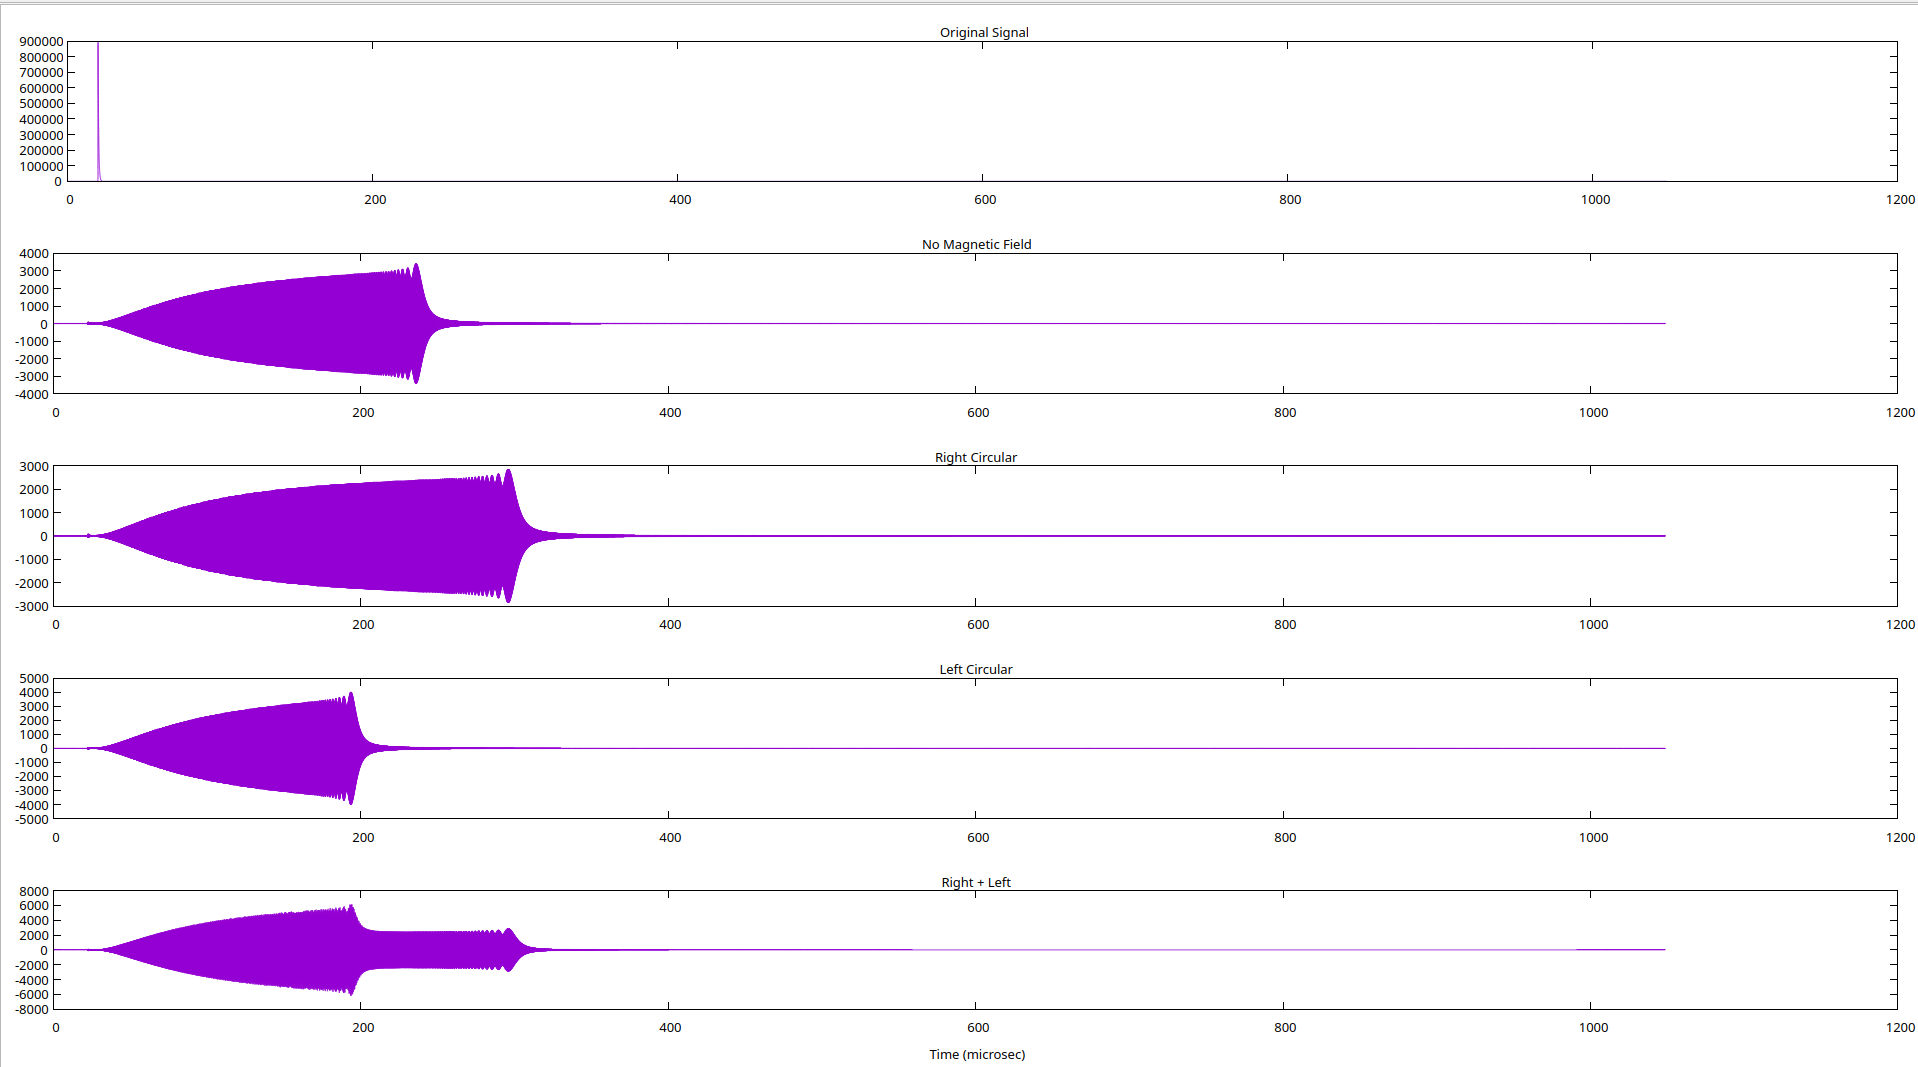
\includegraphics[width= 0.9\textwidth]{signal_stec_15.png}
    \caption{\small The results if the STEC of the atmosphere were half as high. }
    \label{fig:signal-final-results}
\end{figure}

\noindent There is some limitation in what the antennae of an EMP-measuring satellite can analyze.
The sudden taper in the signal is due to the highpass filter put in place, and resembles how satellites measuring EMPs are built to most sensitively receive a certain bandwidth of frequencies.
Furthermore, the antennae can be built to receive the right-circular signal, the left-circular signal, or a sum of both, but not all three at once.

%------------------------------------------------------------------------------------

\section{Limitations}

\noindent Unfortunately, the weather data from the FORTE satellite is not yet publicly available, so I did not have access to real data which would have greatly improved the accuracy of my project.

%------------------------------------------------------------------------------------

\section{Moving Forward}

\noindent Electrons also change the refractive index of the ionosphere, which causes the EMP to change angles, similarly to how light bends when passing through a prism. The extent of this refraction depends on the total electron density of the atmosphere, the wave's frequency, and the angle at which it enters the ionosphere. However, this process does not depend on the phase, so I did not model it.  Moving forward, I would like to plot the data as a spectrogram, take into account refraction, and write a program that calculates the location of each lightning strike.
%-------------------------------------------------------------------------------------------------
\\
\\
\cite{ionosphericdelay} 
\cite{forte}
\cite{edfenimore}
\medskip
\printbibliography
%------------------------------------------------------------------------------------

\end{document}

